
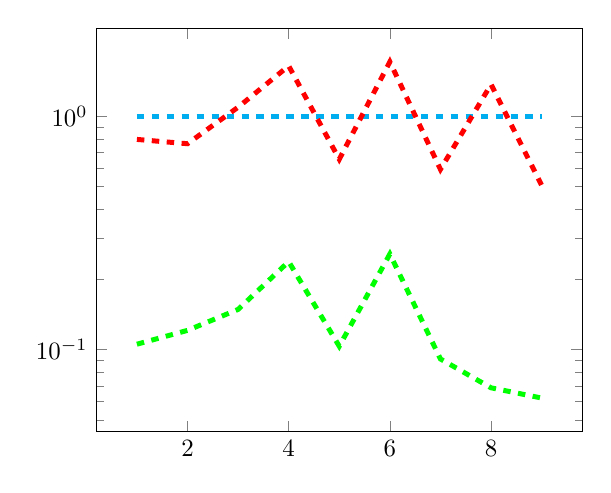
\begin{tikzpicture}[scale=0.9]
\begin{semilogyaxis}
\addplot[dashed,color=cyan,line width=2pt] coordinates {(1,1.0)(2,1.0)(3,1.0)(4,1.0)(5,1.0)(6,1.0)(7,1.0)(8,1.0)(9,1.0)};
\addplot[dashed,color=red,line width=2pt] coordinates {(1,0.7977907604717445)(2,0.7645244181481413)(3,1.0963247011043513)(4,1.6487274584309042)(5,0.655856318894944)(6,1.7167411990597599)(7,0.593484611897854)(8,1.3731673149700505)(9,0.507218196977722)};
\addplot[dashed,color=green,line width=2pt] coordinates {(1,0.10561964074213527)(2,0.12107527552534399)(3,0.14890855718323237)(4,0.23876670618031826)(5,0.10351633457780109)(6,0.25728003073247563)(7,0.09129971435399119)(8,0.0686799446876531)(9,0.06208244585340057)};

\end{semilogyaxis}
\end{tikzpicture}
